%
%  Search for Rare Higgs Decays
%

I begin with a brief discussion of the motivation behind looking for rare Higgs decays like $H \rightarrow \rho+\gamma$ and $H \rightarrow \phi+\gamma$. Then, I outline the event selection methods and relevant backgrounds. Finally, I describe the Boosted Decision tree we used in detail, followed by the results of the analysis.

\begin{section}{Motivation}

The branching ratios for the $H \rightarrow \phi+\gamma$ and $H \rightarrow \rho+\gamma$ decays (see Fig. \ref{fig:whiggs}) are expected to have a lower bound of $8.8 \times 10^{-4}$ and $4.8 \times 10^{-4}$  respectively\cite{cite-rpg-brs}. Put simply, they are \textit{very} rare - so rare, in fact, that they have never been directly observed. Furthermore, by any measure, these decays should never be detectable at human-reachable energies, that is, unless there are yet-undiscovered processes that enhance the rate of either of these decays. This implies that this measurement is experimentally exciting, because any significant measurement of the production of $\rho$ or $\phi$ mesons would be direct evidence of the existence of new physics. At the same time, if no $\rho$ or $\phi$ mesons are found, then the branching ratio of either decay mode can be pushed farther back, depending on the detector's sensitivity to the signature.

\begin{figure}[htb]
\begin{center}
\begin{tikzpicture}
  \begin{feynman}
    \vertex (a1) {\(\overline b\)};
    \vertex[right=1cm of a1] (a2);
    \vertex[right=1cm of a2] (a3);
    \vertex[right=1cm of a3] (a4) {\(b\)};
    \vertex[right=1cm of a4] (a5);
    \vertex[right=2cm of a5] (a6) {\(u\)};

    \vertex[below=2em of a1] (b1) {\(d\)};
    \vertex[right=1cm of b1] (b2);
    \vertex[right=1cm of b2] (b3);
    \vertex[right=1cm of b3] (b4) {\(\overline d\)};
    \vertex[below=2em of a6] (b5) {\(\overline d\)};

    \vertex[above=of a6] (c1) {\(\overline u\)};
    \vertex[above=2em of c1] (c3) {\(d\)};
    \vertex at ($(c1)!0.5!(c3) - (1cm, 0)$) (c2);

    \diagram* {
      {[edges=fermion]
        (b1) -- (b2) -- (a2) -- (a1),
        (b5) -- (b4) -- (b3) -- (a3) -- (a4) -- (a5) -- (a6),
      },
      (a2) -- [boson, edge label=\(W\)] (a3),
      (b2) -- [boson, edge label'=\(W\)] (b3),

      (c1) -- [fermion, out=180, in=-45] (c2) -- [fermion, out=45, in=180] (c3),
      (a5) -- [boson, bend left, edge label=\(W^{-}\)] (c2),
    };

    \draw [decoration={brace}, decorate] (b1.south west) -- (a1.north west)
          node [pos=0.5, left] {\(B^{0}\)};
    \draw [decoration={brace}, decorate] (c3.north east) -- (c1.south east)
          node [pos=0.5, right] {\(\pi^{-}\)};
    \draw [decoration={brace}, decorate] (a6.north east) -- (b5.south east)
          node [pos=0.5, right] {\(\pi^{+}\)};
  \end{feynman}
\end{tikzpicture}
\end{center}
\caption{Feynman diagram\cite{cite-tikz-feynman} for $H \rightarrow \rho+\gamma$ and $H \rightarrow \phi+\gamma$ associated production.}
\label{fig:whiggs}
\end{figure}
\end{section}

\begin{section}{Event Selection}
\begin{subsection}{Data Aquisition}
The analysis begins with data based on a sample of proton-proton collisions collected by the Compact Muon Solenoid (CMS) detector in the LHC. ``Interesting'' events are selected by the first level of the CMS trigger system which uses information from the detector's calorimeters and muon detectors to select events for analysis in a fixed time interval of less than 4 $\mu s$. These events are then further processed by a high-level trigger processor farm, which decreases the event rate from around 100 kHz to less than 1 kHz, before the data is stored. Finally, the particle-flow algorithm reconstructs and identifies all particles from the events selected by the CMS trigger system. With the data properly processed and promptly reconstructed ``online,'' further analysis can be carried out ``offline.''
\end{subsection}
\begin{subsection}{Baseline Selection}
To start offline analysis, we first apply a baseline selection on data and Monte Carlo samples to filter out particularly irrelevant events. First, we require at one ``good" lepton, qualified as:
\begin{itemize}
    \item $p_{T}(\ell^{\pm}) > 10\textnormal{ GeV}$
    \item $\eta(\ell^{\pm}) < 2.4$
    \item $ID(e^{\pm})$ \verb|HAD_medium_noiso_v5|
    \item $ID(\mu^{\pm})$ \verb|isMediumMuonPOG|
    \item $I_{rel}(e^{\pm}) < 0.1$ using \verb|elMiniRelIsoCMS3_EA|
    \item $I_{rel}(\mu^{\pm}) < 0.2$ using \verb|muMiniRelIsoCMS3_EA|
\end{itemize}

\noindent We also require one good photon, qualified as:
\begin{itemize}
    \item $p_{T}(\gamma) > 20\textnormal{ GeV}$
    \item $\eta(\gamma) < 2.5$
    \item $ID(\gamma)$ \verb|isMediumPhotonPOG_Fall17V2|
    \item $I_{rel}(\gamma) < 0.06$
    \item $\Delta R(\gamma, e^{\pm}) < 0.2$
\end{itemize}
\noindent where if two or more good $\ell$ or $\gamma$ candidates are found, the candidate with the highest $p_{T}$ is selected. Finally, we require two, oppositely charged hadrons. This is complicated by the fact that CMS does not distinguish pions and kaons in reconstruction, but we begin by requiring two good hadron ($h$) candidates qualified as:
\begin{itemize}
    \item $p_{T}(h^{\pm}) > 10\textnormal{ GeV}$
    \item $\eta(h^{\pm}) < 2.4$
    \item $0 \geq dz(h^{\pm}) < 0.1$
    \item $I_{rel}(h^{+}+h^{-}) < 0.06$
    \item $\Delta R(h^{+}, h^{-}) < 0.1$
\end{itemize}
\noindent Now, as mentioned previously, the the exact identity of these hadrons is ambiguous. They are saved, by default, as pions, so their four-momenta are all constructed using the pion's mass contribution to the energy component. We add these to form the $\rho$-candidate four-momentum and designate it as the ``pion hypothesis." Then, we manually set the energy-components of the hadron four-momenta using the kaon mass, add them to form the $\phi$-candidate four-momentum, and designate it as the ``kaon hypothesis." If two or more of either hypothesis is found, we select the hypothesis that is closest to the true, respective mass. This leads to the possibility of biasing the data, but we avoid this later by rejecting any events with more than one meson candidate.
\end{subsection}
\end{section}

\begin{section}{Backgrounds}
Lorem ipsum dolor sit amet, consectetur adipiscing elit. Quisque eu eros nisl. Donec sollicitudin nisl nisi, sit amet rutrum nibh faucibus sit amet. In a efficitur dui. Nunc at sagittis urna. Quisque venenatis nec risus quis eleifend. Fusce id nulla in urna tristique iaculis. In et consectetur risus, nec commodo justo. In augue enim, efficitur ac commodo quis, tempus ac arcu. Sed porta dolor ultrices, pellentesque tellus eu, mollis mi. Phasellus et condimentum odio. Curabitur condimentum rhoncus sem, eget sagittis eros rhoncus sit amet. Class aptent taciti sociosqu ad litora torquent per conubia nostra, per inceptos himenaeos. Maecenas ac felis aliquam orci eleifend faucibus vitae sit amet mauris. Fusce vel magna mi. Aenean commodo pellentesque tellus, ut iaculis est auctor et.
Aliquam porttitor justo dolor. Duis ut ex lacinia, vulputate dui a, molestie lorem. Vestibulum elementum lectus vel mollis iaculis. Cras ante purus, pellentesque sit amet sem sed, convallis dapibus est. Aenean vehicula mollis bibendum. Integer aliquet condimentum luctus. Suspendisse vitae rhoncus justo.
\end{section}

\begin{section}{Boosted Decision Tree}
\begin{subsection}{Introduction}
Based on the following basic study, we found that a Boosted Decision Tree (BDT) trained on Monte Carlo simulations of signal and background performed 20\% to 25\% better than traditional, cut-based methods. We determined an optimal BDT working point by sampling the BDT's ROC curve (generated using testing data and predictions) at each defined threshold value, then calculating an expected significance ($\sigma$) defined as:
\begin{equation}
    \sigma = \sqrt{2(s+b)\ln(1+s/b)-2s}
\end{equation}
\noindent where $s$ and $b$ are the number of signal and background events for a given threshold value. The optimal BDT working point is then given by the maximum $\sigma$-value. Next, we defined a general cut-based approach by the following cuts:
\begin{itemize}
    \item $1.0 < m_{\phi} < 1.04$
    \item $\Delta R(K^{+}, K^{-}) < 0.015$
    \item $p_{T}(\phi) > 25\textnormal{ GeV}$
    \item $p_{T}(\gamma) > 40\textnormal{ GeV}$
    \item $I_{rel}(\phi) < 0.01$
\end{itemize}
\noindent Finally, we calculated the false-positive and true-positive rates of the cut-based methods and plotted them against the BDT's ROC curve. The results of this study are plotted in Fig. \ref{fig:bdt-vs-cuts}.

\begin{figure}[htb]
\begin{center}
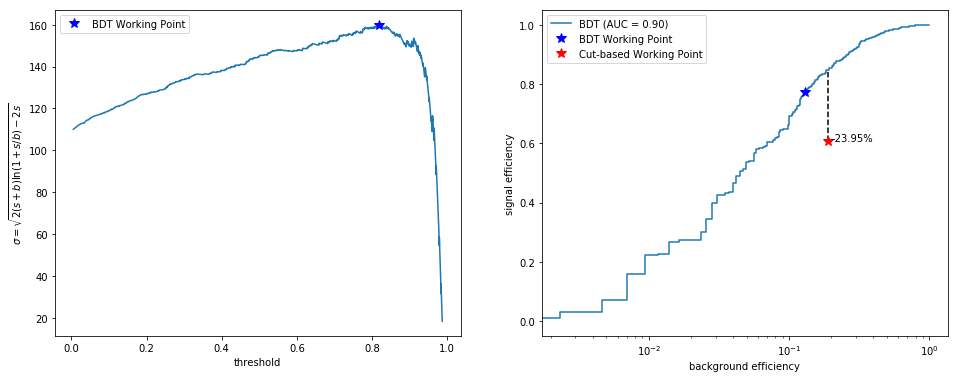
\includegraphics[width=.95\linewidth]{Dissertation/fig/bdt-vs-cuts.png}
\end{center}
\caption{Left: Expected significance ($\sigma$) versus BDT threshold value. Right: Comparison between an optimal BDT working point and cut-based method plotted on top of the BDT's ROC curve.}
\label{fig:bdt-vs-cuts}
\end{figure}
\end{subsection}
\begin{subsection}{Training}
We began with the XGBoost python package, a well-known implementation of gradient-boosted decision trees. Twenty-two features were selected, from those saved during the baseline selection step, based on their merit as variables that are reasonably uncorrelated to the signal region (reconstructed Higgs boson mass). The unweighted distributions for all input features are shown in Fig. \ref{fig:bdt-vars}, but they are also listed below divided into categories for brevity and later reference:
\begin{enumerate}[(i.)]
    \item Missing Transverse Energy ($\slashed{E}_{T}$):
    \begin{itemize}
        \item $p_{T}(\slashed{E}_{T})$
        \item $\varphi(\slashed{E}_{T})$
    \end{itemize}
    \item Basic Kinematics:
    \begin{itemize}
        \item $p_{T}(\gamma)$, $p_{T}(\phi)$
        \item $\eta(\gamma)$, $\eta(\phi)$, $\eta(\ell^{\pm})$
        \item $\varphi(\gamma)$, $\varphi(\phi)$, $\varphi(\ell^{\pm})$
        \item $\Delta R(\gamma, \ell^{\pm})$, $\Delta R(\phi, \gamma)$, $\Delta R(K^{+}, K^{-})$
    \end{itemize}
    \item Masses:
    \begin{itemize}
        \item $m_{Z}$, $m_{\phi}$
    \end{itemize}
    \item MELA ``Magic" Angles:
    \begin{itemize}
        \item $\Phi$, $\Phi_{1}$
        \item $\cos\theta_{1}$, $\cos\theta_{2}$, $\cos\theta^{*}$
    \end{itemize}
\end{enumerate}

\noindent There are some important clarifications to make here. First, we scaled all $p_{T}$ quantities that are correlated to the Higgs and input into the BDT by the Higgs mass. Second, $\varphi$ refers to the azimuthal angle (see Fig. \ref{fig:cms-coords}) which is not to be confused with the $\phi$-meson. Finally, we calculated the quantities listed under (.iv) using MELA\cite{cite-mela} (all angles used are illustrated in Fig. \ref{fig:magic-angles}).

\begin{figure}[htb]
\begin{center}
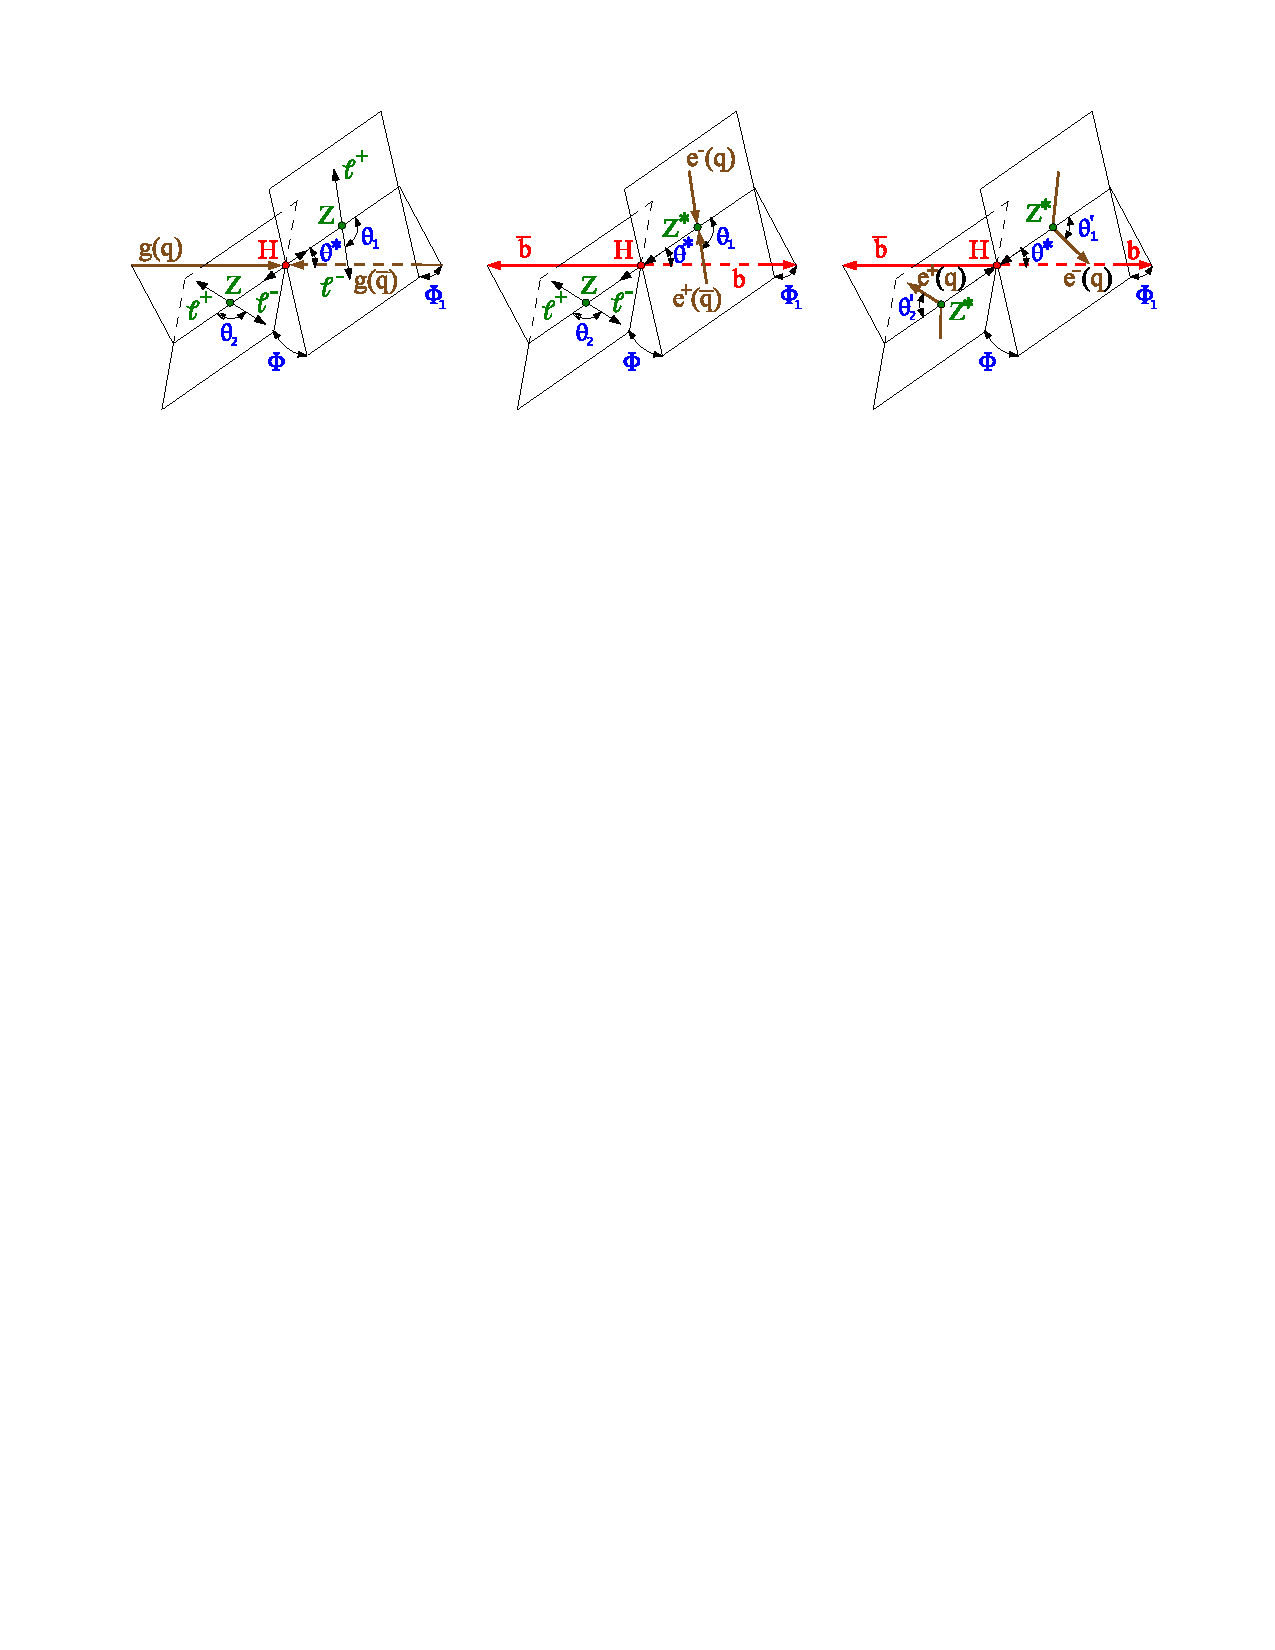
\includegraphics[width=.95\linewidth]{Dissertation/fig/magic-angles.pdf}
\end{center}
\caption{Diagram due to Anderson et. al. \cite{magic-angles-cite} of Higgs-frame angles used for BDT training. The center diagram is most relevant under the following replacements: $Z, Z^*$ to $W, W^*$, $b, \bar{b}$ to $\rho/\phi, \gamma$; $\ell^+,\ell^-$ to $e^-/\mu^-, \nu_e/ \nu_\mu$.}
\label{fig:magic-angles}
\end{figure}

\begin{figure}[htb]
\begin{center}
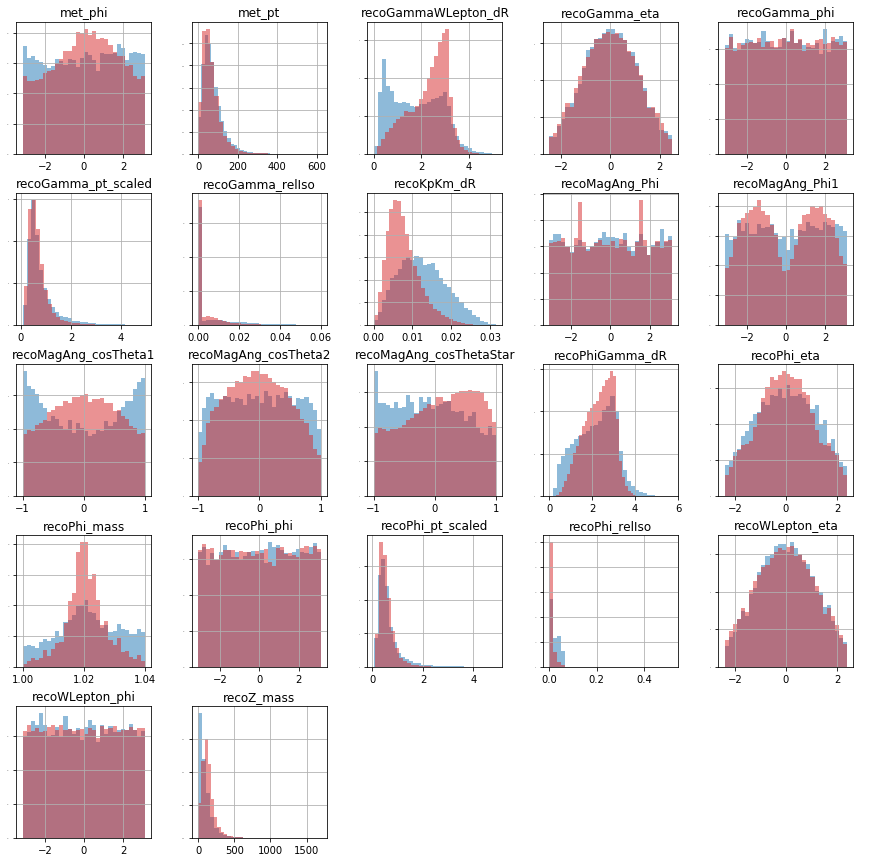
\includegraphics[width=.95\linewidth]{Dissertation/fig/bdt-training.png}
\end{center}
\caption{Preliminary histograms for every feature used to train the BDT. These were drawn before any weights are applied, so they do not completely represent what the BDT saw, however they do provide some insight into the motivation behind the BDT's variable rankings.}
\label{fig:bdt-training}
\end{figure}
\end{subsection}
\begin{subsection}{Performance}
Aliquam porttitor justo dolor. Duis ut ex lacinia, vulputate dui a, molestie lorem. Vestibulum elementum lectus vel mollis iaculis. Cras ante purus, pellentesque sit amet sem sed, convallis dapibus est. Aenean vehicula mollis bibendum. Integer aliquet condimentum luctus. Suspendisse vitae rhoncus justo. Aliquam porttitor justo dolor. Duis ut ex lacinia, vulputate dui a, molestie lorem. Vestibulum elementum lectus vel mollis iaculis. Cras ante purus, pellentesque sit amet sem sed, convallis dapibus est. Aenean vehicula mollis bibendum. Integer aliquet condimentum luctus. Suspendisse vitae rhoncus justo. Aliquam porttitor justo dolor. Duis ut ex lacinia, vulputate dui a, molestie lorem. Vestibulum elementum lectus vel mollis iaculis. Cras ante purus, pellentesque sit amet sem sed, convallis dapibus est. Aenean vehicula mollis bibendum. Integer aliquet condimentum luctus. Suspendisse vitae rhoncus justo. Aliquam porttitor justo dolor. Duis ut ex lacinia, vulputate dui a, molestie lorem. Vestibulum elementum lectus vel mollis iaculis. Cras ante purus, pellentesque sit amet sem sed, convallis dapibus est. Aenean vehicula mollis bibendum. Integer aliquet condimentum luctus. Suspendisse vitae rhoncus justo.

\begin{figure}[htb]
\begin{center}
\begin{tabular}{llll}
\toprule
cut &       gain &       cover &  weight \\
\midrule
$I_{rel}(\phi)$ &  64.823995 &  410.500067 &      57 \\
$\Delta R(K^{+}, K^{-})$ &  49.762952 &  315.353542 &     143 \\
$m_{Z}$ &  34.554528 &  292.716951 &     107 \\
$p_{T}(\phi)$ &  30.415027 &  256.183022 &     123 \\
$m_{\phi}$ &  21.122510 &  374.886933 &      79 \\
$\Delta R(\phi, \gamma)$ &  15.631570 &  256.192849 &     100 \\
$p_{T}(\gamma)$ &  13.298290 &  179.156460 &      46 \\
$\cos\theta_{1}$ &  10.042543 &  346.471954 &      58 \\
$I_{rel}(\gamma)$ &   9.113523 &  269.280112 &      38 \\
$\cos\theta^{*}$ &   7.324339 &  188.648235 &      52 \\
\bottomrule
\end{tabular}

\end{center}
\caption{Top ten variables as ranked by the BDT by gain. All input variables are reconstruction-level Monte Carlo data, and all $p_{T}$ variables are scaled by $m_{H}.$}
\label{fig:bdt-vars}
\end{figure}

\begin{figure}[htb]
\begin{center}
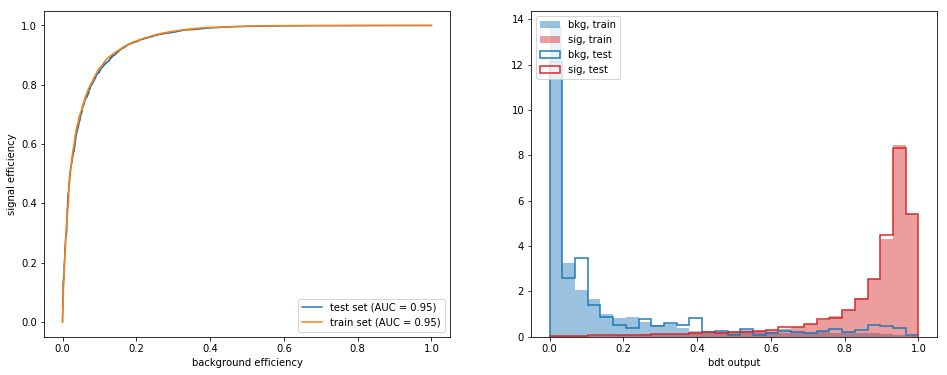
\includegraphics[width=.95\linewidth]{Dissertation/fig/bdt-performance.png}
\end{center}
\caption{Left: ROC curve showing BDT testing (blue) and training (orange) performance. Right: Background (blue) and signal (red) distributions versus BDT score for testing (outline) and training (filled).}
\label{fig:bdt-performance}
\end{figure}
\end{subsection}

\begin{subsection}{Validation}
Aliquam porttitor justo dolor. Duis ut ex lacinia, vulputate dui a, molestie lorem. Vestibulum elementum lectus vel mollis iaculis. Cras ante purus, pellentesque sit amet sem sed, convallis dapibus est. Aenean vehicula mollis bibendum. Integer aliquet condimentum luctus. Suspendisse vitae rhoncus justo.

\begin{figure}[htb]
\begin{center}
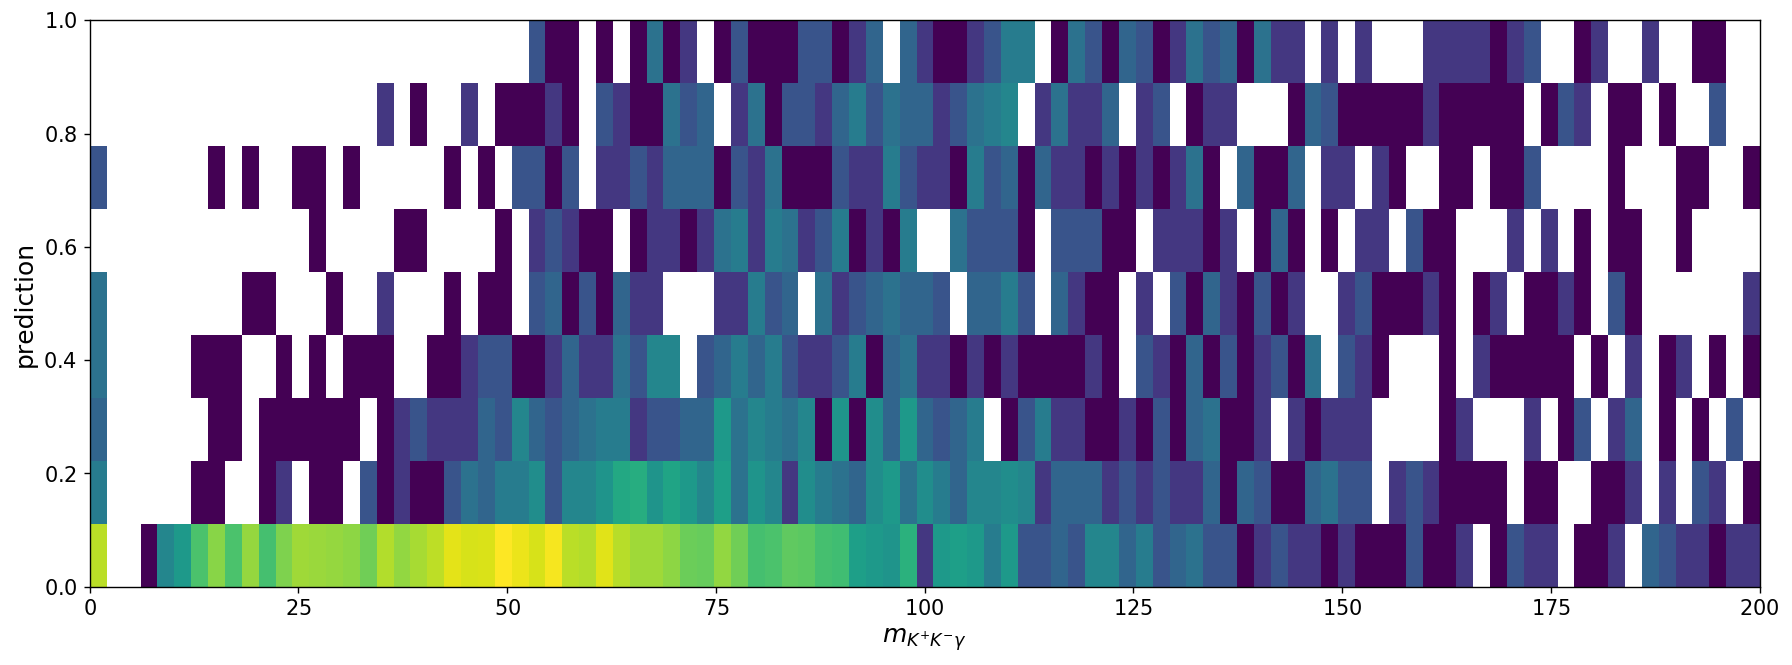
\includegraphics[width=.95\linewidth]{Dissertation/fig/bdt-bkgsculpt1.png}
\end{center}
\caption{Plot of the BDT score versus the reconstructed Higgs mass. A heavy correlation between high score and the true Higgs mass would suggest background is being sculpted.}
\label{fig:bdt-bkgsculpt1}
\end{figure}

\begin{figure}[htb]
\begin{center}
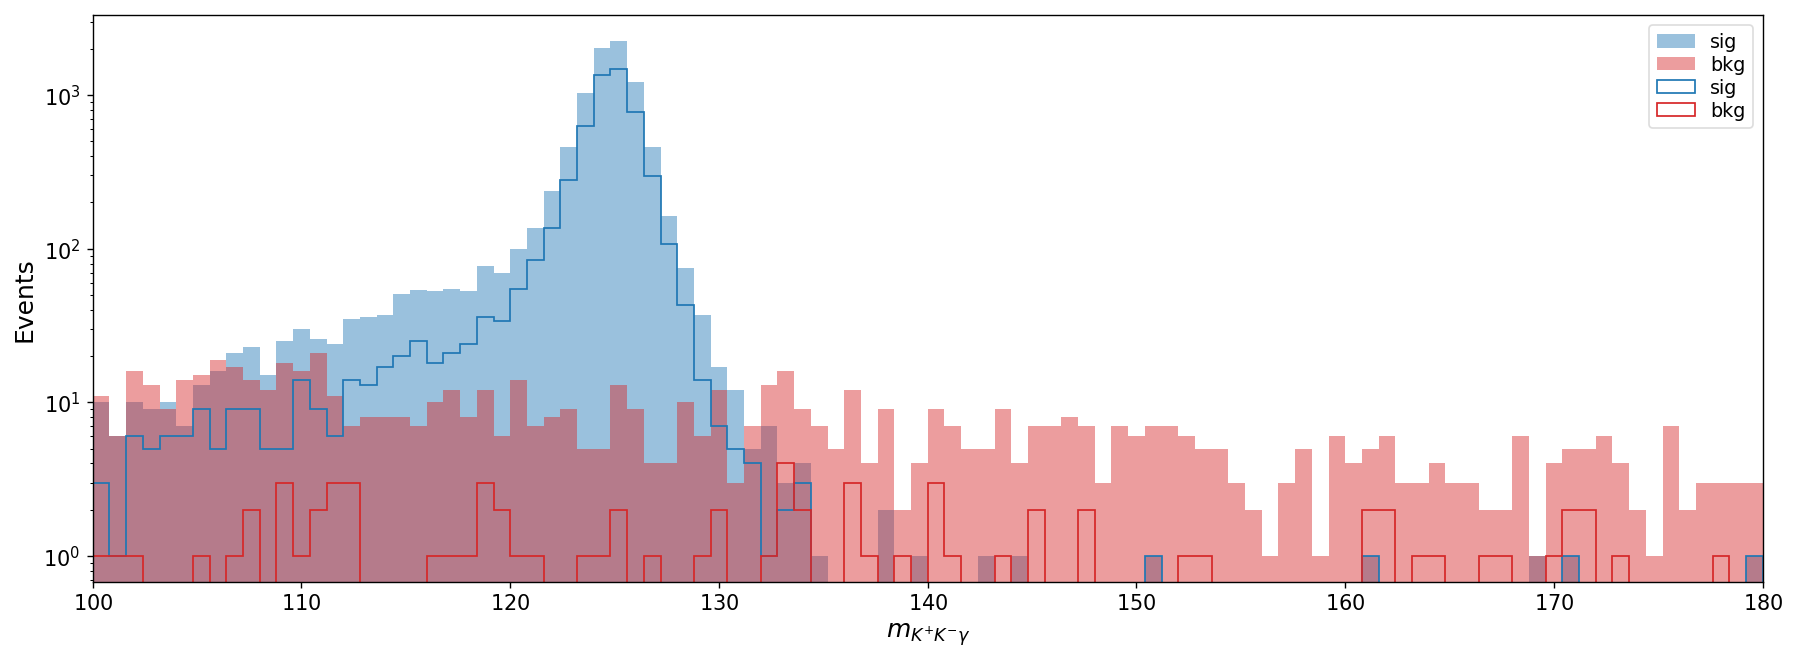
\includegraphics[width=.95\linewidth]{Dissertation/fig/bdt-bkgsculpt2.png}
\end{center}
\caption{Reconstructed Higgs mass distribution for signal (blue) and background (red) before (filled) and after (outline) requiring $D > 0.9$ where $D$ is the BDT discriminant.}
\label{fig:bdt-bkgsculpt2}
\end{figure}
\end{subsection}
\end{section}

\begin{section}{Results}

Lorem ipsum dolor sit amet, consectetur adipiscing elit. Quisque eu eros nisl. Donec sollicitudin nisl nisi, sit amet rutrum nibh faucibus sit amet. In a efficitur dui. Nunc at sagittis urna. Quisque venenatis nec risus quis eleifend. Fusce id nulla in urna tristique iaculis. In et consectetur risus, nec commodo justo. In augue enim, efficitur ac commodo quis, tempus ac arcu. Sed porta dolor ultrices, pellentesque tellus eu, mollis mi. Phasellus et condimentum odio. Curabitur condimentum rhoncus sem, eget sagittis eros rhoncus sit amet. Class aptent taciti sociosqu ad litora torquent per conubia nostra, per inceptos himenaeos. Maecenas ac felis aliquam orci eleifend faucibus vitae sit amet mauris. Fusce vel magna mi. Aenean commodo pellentesque tellus, ut iaculis est auctor et.

\end{section}